\documentclass[12pt]{report}
\title{System validation document}
\date{\today \\ Version 0.0.1}

\usepackage[latin1]{inputenc}
\usepackage{amsmath}
\usepackage{graphicx}
\usepackage{a4wide}
\usepackage{enumitem}
\usepackage{url}
\usepackage{caption}
\usepackage[parfill]{parskip}
\usepackage{appendix}
\usepackage{subcaption}
\usepackage{color}
\usepackage{booktabs}
\usepackage{lineno}
\usepackage{float}
\usepackage{longtable}
\usepackage{colortbl}
\usepackage{amsfonts}
\newcounter{counter}

%\linenumbers
\modulolinenumbers[5]

\begin{document}
	\begin{titlepage}
		\begin{center}
			\textsc{\Large EINDHOVEN UNIVERSITY OF TECHNOLOGY}\\[1.5cm]
			
			\textsc{\Large System Validation}\\[0.8cm]
			\hrule
			\vspace{0.5cm}
			{ \huge \bfseries EUV Wafer Stepper \\[0.4cm] }
			\hrule
			\vspace{1.5cm}
			\noindent
			\begin{minipage}[t]{0.5\textwidth}
				\begin{flushleft} \large
					\emph{Authors:}\\
					R.M. van den Hurk (0817761)\\
					Z. Ben Snaiba (0748095)\\
					P.M.M. van Wesel (0818131)\\
				\end{flushleft}
			\end{minipage}\\
			\vspace{5cm}
			\begin{minipage}[t][8cm]{0.3\textwidth}
				\begin{flushright} \large
					\today
				\end{flushright}
			\end{minipage}
			
			\vfill
			
		\end{center}
	\end{titlepage}
	
	\tableofcontents
	
	\chapter{System overview}
	
	\section{Global overview}
	A global overview of the system.
	
	\chapter{System requirements}
	
	\newcommand{\req}[1]{
		\item[\textbf{R\stepcounter{counter}\arabic{counter}}] {#1}
		\hrule
	}
	
	\newcommand{\reqb}[2]{
		\item[\textbf{{#1}}] {#2}
		\hrule
	}
	
	\section{Liveness requirement}
	\begin{itemize}
		\req{If the system is operating normally, an untreated wafer on the input rack will enter the system, and exit the system after it has been treated.}
	\end{itemize}
	
	\section{Sluice requirements}
	\begin{itemize}
		\req{Only one sluice door can be open at a time.}
		\req{The outer sluice door can only open if there is normal air pressure inside the sluice.}
		\req{The inner sluice door can only open if there is a vacuum inside the sluice.}
		\req{The vacuum pump can only make a vacuum if both sluice doors are closed.}
		\req{The doors of a sluice can not close if a robot is reaching inside.}
	\end{itemize}
	
	\section{Sluice robot requirements}
	\begin{itemize}
		\req{Robot A may only move to a sluice if the outer door of the target sluice is open.}
		\req{Robot B may only move to a sluice if the inside door of the target sluice is open.}
		\req{Robot A\&B may only choose a sluice to put a wafer in that is empty.}
		\req{Robot A\&B may only try to retrieve a wafer from an occupied sluice.}
		\req{Robot A\&B can only put a wafer on an empty spot on the rack.}
		\req{Robot A\&B may only target functioning sluices.}
		\req{Robot A\&B should only try to take wafers from the rack if there are wafers available.}
		\req{Robot B may not access the same spot on the rack as Robot C at the same time.}
	\end{itemize}
	
	\section{Inside robot requirements}
	\begin{itemize}
		\req{Robot C can not access the same spot on the rack as Robot B at the same time.}
		\req{If there is no wafer on the projection platform Robot C should try to take a wafer from the rack and place it on the projection platform.}
		\req{Robot C can not put a wafer on the projection platform when it is occupied.}
		\req{Robot C can not take a wafer from the projection platform if the projection is not done.}
		\req{If the projection is done, Robot C should take the wafer from the projection platform.}
		\req{Robot C can not put a wafer on an occupied place on the rack.}
	\end{itemize}
		
	\section{Projector requirements}
	\begin{itemize}
		\req{The projector only starts its treatment when a wafer is on the projection platform.}
	\end{itemize}
	
	\chapter{System interactions}
\section{User actions}
	\begin{itemize}
\item openOuterDoor(N) - Open the outer door of sluice N.
\item closeOuterDoor(N) - Close the outer door of sluice N.
\item openInnerDoor(N) - Open the inner door of sluice N.
\item closeInnerDoor(N) - Close the inner door of sluice N.
\item pumpVacuum(N) - Make a vacuum in sluice N.
\item releaseVacuum(N) - Release the vacuum in sluice N.
\item robotTakeWafer(R, P) - Robot R picks up a wafer from its input rack from position P.
\item robotDepositWafer(R, P) - Robot R deposits the wafer it is holding wafer on its output rack from position P.
\item robotWaferInSluice(R, N) - Robot R puts the wafer it is holding wafer in sluice N.
\item robotWaferFromSluice(R, N) - Robot R takes a wafer from sluice N.
\item robotCTreatWafer - Robot C puts the wafer it is holding on the projector.
\item robotCRetrieveWafer - Robot C takes the wafer from the projector.
\item treatWafer - The projector treats a wafer.
\end{itemize}

	\section{System events}
	\begin{itemize}
\item outerDoorOpen(N) - True if the outer door of sluice N is open false otherwise.
\item innerDoorOpen(N) - True if the outer door of sluice N is open false otherwise.
\item vacuum(N) - True if there is currently a vacuum in sluice N false otherwise.
\item waferInSluice(N) - True if there is a wafer is sluice N false otherwise
\item robotInSluice(N) - True if there is a robot in sluice N false otherwise
\item robotAccessingRack(R, N) -  True if robot R is currently accesing rack N.
\item waferOnRack(R, P) - True if there is a wafer in rack R at position P false otherwise
\item waferTreated - True if the wafer in the projector has been treated false otherwise
\item sluiceBroken(N) - Sluice N has failed to respond to a user action and will be marked as broken.
\item waferInProjector - Whether there is a wafer in projector or not.
	\end{itemize}
	
	\chapter{Requirements in terms of interactions}
	\section{Liveness requirement}
	\begin{itemize}
		\reqb{SR1}{If a wafer appears at position p on the input rack, we should see the following sequence of actions. Other actions can happen between any two of these actions, provided they are not one of those two actions with different parameters.\\
		\begin{itemize}
\item robotTakeWafer( A, p )
\item robotWaferInSluice( A, s ) \emph{- For some arbitrary sluice s}
\item robotWaferFromSluice( B, s )
\item robotDepositWafer( B, p2 ) \emph{- For some arbitrary position p2 on the inner} rack.
\item robotTakeWafer( C, p2 ) \emph{directly followed by} robotCTreatWafer.
\item robotDepositWafer( C, p3 ) \emph{- For some arbitrary position p3 on the inner rack.}
\item robotTakeWafer( B, p3 )
\item robotWaferInSluice( B, s2 ) \emph{- For some arbitrary sluice s2.}
\item robotWaferFromSluice( A, s2 )
\item robotDepositWafer( A, p4 ) \emph{- For some arbitrary position p4 on the output rack.}
\end{itemize}
}
	\end{itemize}
	
	\section{Sluice requirements}
	\begin{itemize}
		\reqb{SR2}{openOuterDoor(N) if innerDoorOpen(N) is true.}
		\reqb{SR3}{openOuterDoor(N) vacuum(N) is false.}
		\reqb{SR4}{openInnerDoor(N) vacuum(N) is true.}
		\reqb{SR5}{pumpVacuum(N) outerDoorOpen(N) and innerDoorOpen(N) are both true.}
		\reqb{SR6}{
\begin{itemize}		
		\item closeOuterDoor(N) can only happen if robotInSluice(N) is false.
\item closeInnerDoor(N) can only happen if robotInSluice(N) is false.
\end{itemize}		
		}
	\end{itemize}
	
	\section{Sluice robot requirements}
	\begin{itemize}
		\reqb{SR7}{robotWaferInSluice(A,N) can only happen if outerDoorOpen(N) is true.}
		\reqb{SR8}{robotWaferInSluice(B,N) can only happen if innerDoorOpen(N) is true.}
		\reqb{SR9}{\begin{itemize}
		\item  robotWaferInSluice(A, N) waferInSluice(N) is false.
		\item robotWaferInSluice(B, N) waferInSluice(N) is false.
		\end{itemize}}
		\reqb{SR10}{
		\begin{itemize}
		\item robotWaferFromSluice(A, N) can only happen if  waferInSluice(N) is true
		\item robotWaferFromSluice(B, N) can only happen if waferInSluice(N) is true.
		\end{itemize}
		}
		\reqb{SR11}{?}
		\reqb{SR12}{openOuterDoor(N), closeOuterDoor(N), openInnerDoor(N), closeInnerDoor(N), pumpVacuum(N), releaseVacuum(N), robotWaferInSluice(R,N),robotWaferFromSluice(R,N),outerDoorOpened(N), outerDoorClosed(N),innerDoorOpened(N),innerDoorClosed(N),vacuumDone(N) and vacuumReleased(N) can only happen if sluiceBroken(N) is false.}
		\reqb{SR13}{?}
		\reqb{SR14}{RobotTakeWafer(B, p) or RobotDepositWafer(B, p) can only happen if robotAccessingRack(C,C\_Rack) is false.}	\end{itemize}
	
	\section{Inside robot requirements}
	\begin{itemize}
		\reqb{SR15}{RobotTakeWafer(C, p) or RobotDepositWafer(C, p) can only happen if robotAccessingRack(B,C\_Rack) is false. }
		\reqb{SR16}{should?}
		\reqb{SR17}{robotCRetreiveWafer can only happen if waferInProjector is false.}
		\reqb{SR18}{robotCRetreiveWafer can only happen if waferTreated is true.}
		\reqb{SR19}{should?}
		\reqb{SR20}{robotDepositWafer(C, N) can only happen if waferOnRack(C\_Rack, P) is true for some P.}
	\end{itemize}
	\section{Projector requirements}
	\begin{itemize}
		\reqb{SR21}{treatWafer can only happen after robotCTreatWafer if no robotCRetrieve happened after that.}
	\end{itemize}
	
	\chapter{System model}
	\section{Schematic overview}
	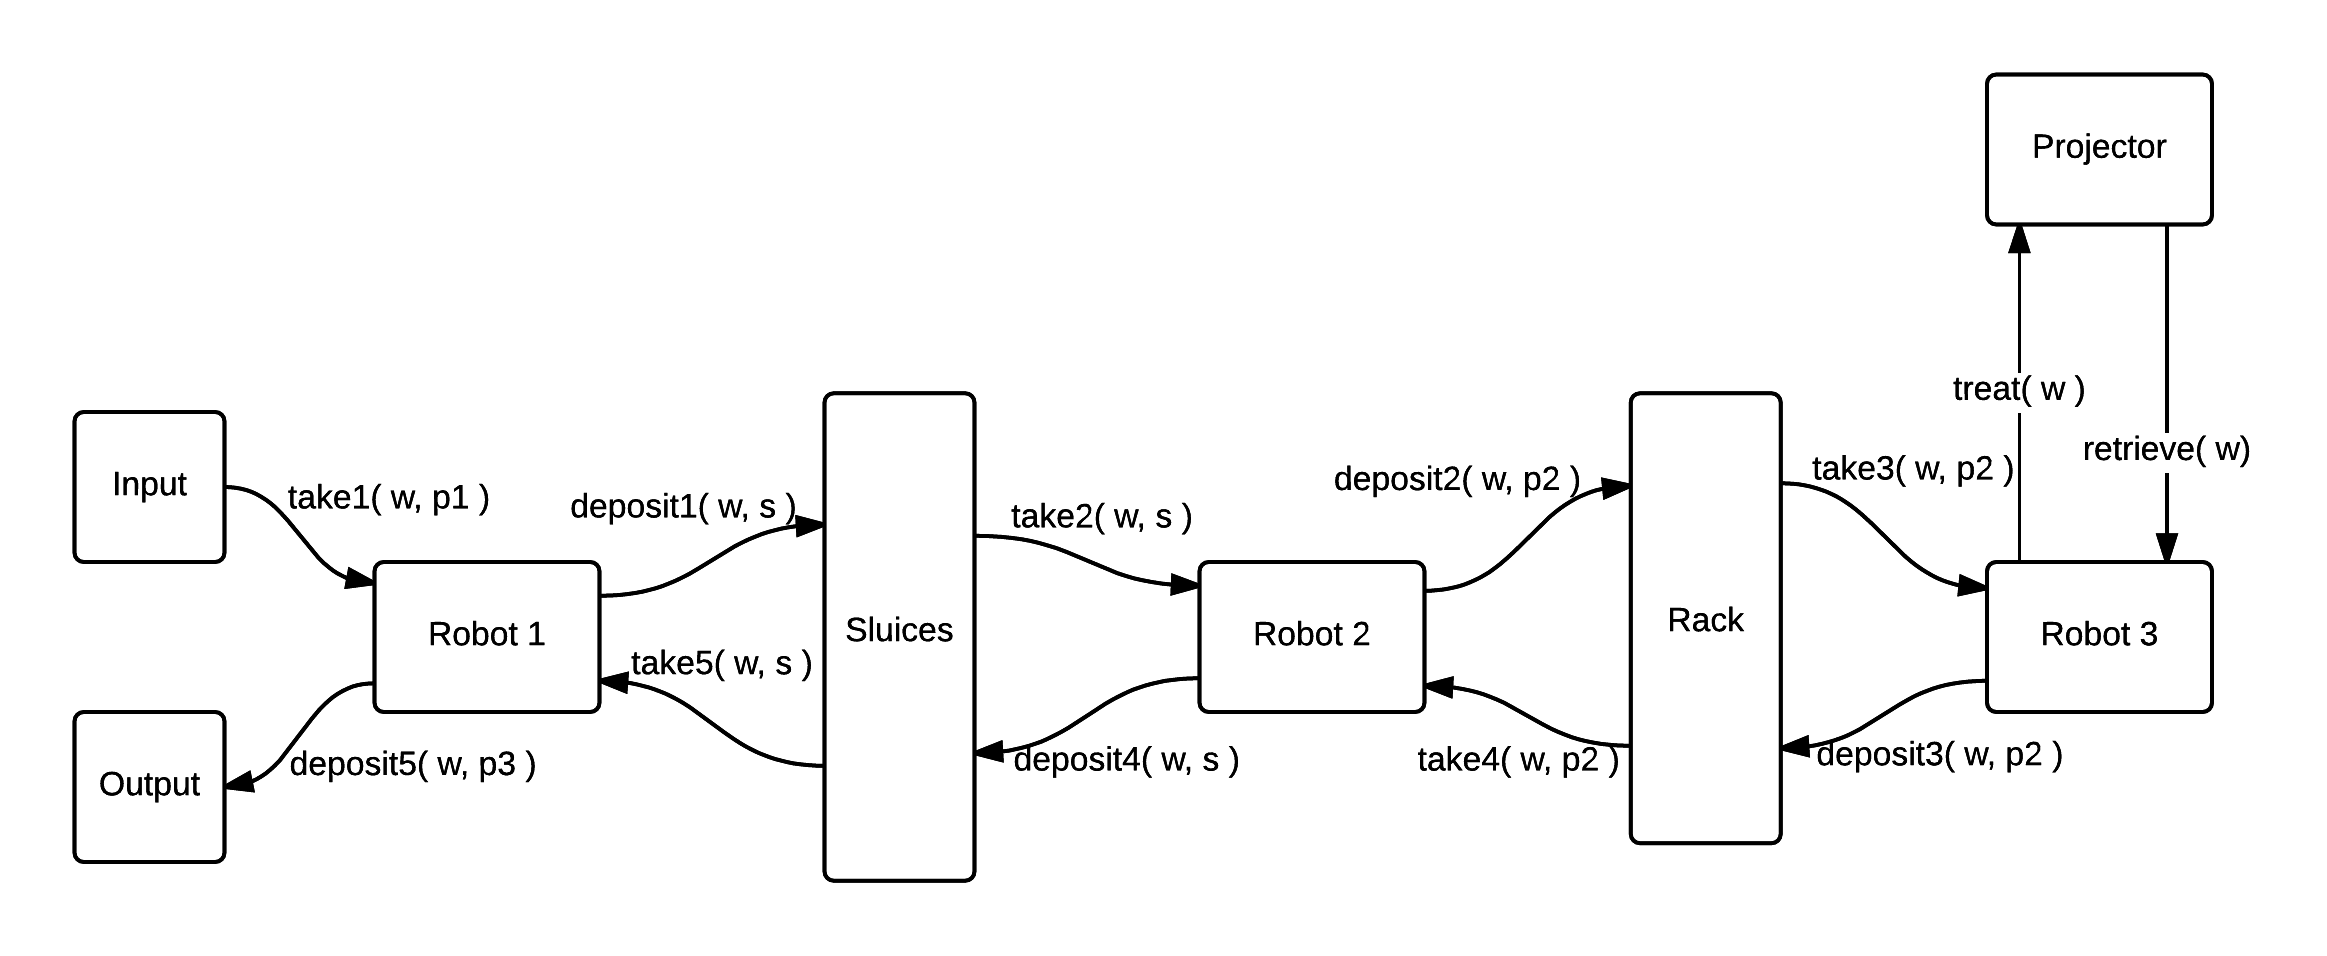
\includegraphics[scale=0.9]{modelschema}
	
	\section{Formal model}
	\textbf{sort}\\
		Id = $\mathbb{N}$\\
		Wafer = struct $w_1 | w_2$\\
		p1, p2, p3 = $\mathbb{N}$\\
		
	\textbf{something}\\
		Robot 1 = $\sum\nolimits_{p_1 \in Input} take1( w_1, p_1 ) \cdot \sum\nolimits_{s \in Sluices} deposit1( w_1, s ) +$\smallskip\\ 
		\- \hspace{4.3em} $\sum\nolimits_{s \in Sluices} take5( w_2, s ) \cdot \sum\nolimits_{p_3 \in Output} deposit5( w_2, p_3 )$\bigskip\\
		Robot 2 = $\sum\nolimits_{s \in Sluices} take2( w_1, s ) \cdot \sum\nolimits_{p_2 \in Rack} deposit2( w_1, p_2 ) +$\smallskip\\ 
		\- \hspace{4.3em} $\sum\nolimits_{p_2 \in Rack} take4( w_2, p_2 ) \cdot \sum\nolimits_{s \in Sluices} deposit4( w_2, s )$ \bigskip\\
		Robot 3 = $\sum\nolimits_{p_2 \in Rack} take3( w_1, p_2 ) \cdot treat( w_1 ) +$\smallskip\\ 
		\- \hspace{4.3em} $retrieve( w_2 ) \cdot \sum\nolimits_{p_2 \in Rack} deposit4( w_2, p_2 )$\bigskip\\
		Projector = $treat( w_1 ) \cdot treatWafer \cdot retrieve( w_1 )$

\end{document} 